\documentclass[12pt,a4paper]{article}

\usepackage[utf8]{inputenc}
\usepackage[T1]{fontenc}
\usepackage{lmodern}
\usepackage[margin=2.5cm]{geometry}
\usepackage{amsmath,amssymb}
\usepackage{graphicx}
\usepackage{booktabs}
\usepackage{hyperref}
\usepackage{natbib}
\usepackage{setspace}
\usepackage{xcolor}
\usepackage{float}
\usepackage{caption}

\hypersetup{
    colorlinks=true,
    linkcolor=blue!60!black,
    citecolor=blue!60!black,
    urlcolor=blue!60!black
}

\onehalfspacing

\title{%
  \textbf{UK Ethnic Demographic Change Under Alternative}\\[0.3em]
  \textbf{Migration and Demographic Scenarios, 2022--2122}\\[1em]
  \large Conditional Projections for England and Wales from Census 2021\\
  and ONS 2022-Based Assumptions
}

\author{Scott Brodie Forsyth}
\date{July 2026}

\begin{document}

\maketitle

\begin{abstract}
\noindent
This paper presents an open, reproducible population-projection system for examining how
the self-identified ethnic composition of the United Kingdom could evolve under alternative
demographic assumptions over a 100-year horizon. The system implements a multistate
cohort-component model with separate immigration and emigration, age-specific fertility and
mortality, and a five-category migrant-generation state space. The central estimand is the
\emph{conditional demographic trajectory} generated by a specified set of assumptions---not
a prediction of future population composition.

The first empirical application covers England and Wales. The mid-2022 base population of
60.3 million is constructed from Census 2021 ethnicity tables (ONS RM032), disaggregated to
single year of age using official mid-year population estimates, and scaled to ONS mid-2022
totals. Mortality follows ONS National Life Tables (2020--2022); fertility is calibrated
from Nomis live-birth registrations (2022) and Census ethnic fertility differentials;
migration volumes follow ONS 2022-based national population projection variants (zero, low,
principal, and high net international migration), with age and ethnic profiles derived from
Census country-of-birth tables.

Under the principal ONS migration variant, the model projects 64.9 million residents in
England and Wales by 2050, with the White share in England falling from 81.0\% (2022) to
66.3\%; under the high-migration variant, population reaches 72.7 million with a White share
of 63.5\%. Under zero net migration, population falls to 52.7 million by 2050. All outputs are
conditional on stated assumptions; century-scale trajectories require hindcast validation
before substantive interpretation. Extension to Scotland and Northern Ireland, historical
hindcasts, probabilistic uncertainty, and partnership-based fertility remain future work.
\end{abstract}

\vspace{1em}
\noindent\textbf{Keywords:} population projection, ethnicity, migration, cohort-component model,
England and Wales, demographic scenarios, Census 2021

\section{Introduction}

Population projections by ethnic group are analytically important and methodologically
demanding. Ethnicity in the United Kingdom is measured through self-identification on the
census; categories have changed across census rounds; and the demographic behaviour associated
with ethnic groups---fertility, mortality, migration, partnership, and identity
transmission---differs in ways that standard national projections do not capture
\citep{haskey2002, rees2011, rees2017}.

Prior work demonstrates both the feasibility and the sensitivity of long-run ethnic
composition trajectories to assumptions about fertility convergence and migration, including
\citet{wohland2010}, \citet{coleman2010}, and the \textsc{NewEthPop} system
\citep{newethpop}. This work extends that tradition with an open-source pipeline updated
for Census 2021 base populations, explicit preregistration of scenarios in version-controlled
YAML files, separate immigration and emigration modules, and parameter calibration from
official aggregate tables rather than synthetic demonstration values.

The research question, stated at UK level, is:

\begin{quote}
\emph{How does the projected ethnic composition of the United Kingdom change between 2022
and 2122 under alternative migration and demographic scenarios?}
\end{quote}

The answer is always conditional: under assumptions $A$, the model produces trajectory $T_A$.
The system never claims that ``the UK will have'' a particular ethnic composition. Outputs
are labelled accordingly throughout. The present implementation reports results for England
and Wales; extension to Scotland and Northern Ireland follows the same architecture once
harmonised census bases are integrated.

\subsection{Contributions}

This paper makes four contributions. First, it specifies a transparent multistate
cohort-component architecture for ethnic population projection with documented accounting
identities. Second, it implements reproducible ingestion of Census 2021 and ONS/Nomis
aggregate tables for England and Wales, with version-controlled ethnic harmonisation.
Third, it calibrates mortality, fertility, and migration parameters from official sources,
including ONS 2022-based national population projection (NPP) migration variants
\citep{ons2024nppvariants}. Fourth, it reports conditional scenario results to 2122 under
those assumptions---with explicit validation caveats---illustrating how migration volume
affects both population scale and ethnic composition.

\subsection{Scope and remaining limitations}

Geographic coverage is currently England and Wales only. Scotland (Census 2022) and
Northern Ireland (Census 2021) are not yet integrated. Parental country-of-birth tables are
not yet linked, so UK-born persons with foreign-born parents cannot be distinguished from
those with two UK-born parents. Partnership-weighted fertility and census-estimated child
ethnicity assignment remain rule-based approximations pending linkage to census household
and parental-ethnicity tables. Fertility convergence by duration of residence is specified
but not yet applied in the projection engine. Migration long-term volumes from ONS NPP are
applied as constant annual flows from the first projection step (mid-2022 to mid-2023); the
ONS transition path to long-term assumptions over 2022--2028 is not yet implemented.
Mortality is held at the 2020--2022 period schedule with no projected improvement; fertility
schedules are static after calibration. Realized emigration may fall below the assumed outflow
when age-specific stocks are insufficient (flows are capped at available population). Aggregate
England and Wales population totals are not benchmarked to ONS principal NPP population
outputs, which incorporate mortality improvement and other features not yet modelled here.
No historical hindcast has been completed; outputs to 2122 should not be interpreted as
forecasts until validation against Census 2011 and 2021 is reported.

\section{Conceptual framework}

\subsection{Ethnicity as self-identified and changeable}

Ethnicity is treated as a self-identified social category, distinct from nationality,
citizenship, religion, ancestry, and country of birth \citep{ons2021ethnicity, ons2023rm032}.
A person may report a different ethnic identity at different censuses. Country of birth is
not used as a direct proxy for ethnicity; it informs migrant-generation classification only,
with the relationship documented in the harmonisation metadata.

\subsection{Population state space}

The population at year $t$ is represented as:
\begin{equation}
    N_{n,e,g,s,a,t}
    \label{eq:state}
\end{equation}
where $n$ indexes UK nation, $e$ ethnic group, $g$ migrant generation, $s$ sex, and $a$ age
(0--100+). Generation categories are:
\begin{enumerate}
    \item foreign-born, arrived as adult;
    \item foreign-born, arrived as child;
    \item UK-born with two foreign-born parents;
    \item UK-born with one foreign-born parent;
    \item UK-born with two UK-born parents.
\end{enumerate}
Generation is not inferred from ethnicity alone. In the current England/Wales base,
generation shares within each ethnic group are assigned from Census 2021 tables RM010
(ethnic group by country of birth) and RM011 (country of birth by age).

\subsection{Geographic scope}

England and Wales are modelled as separate nations with zero net internal migration in the
current implementation. Scotland and Northern Ireland will be added when harmonised census
bases are available. Census day was 21 March 2021; the projection base year is mid-2022,
with counts adjusted using ONS mid-year population estimates.

\section{Projection model}

\subsection{Cohort-component transition}

For existing cohorts, the core transition equation is:
\begin{equation}
    N_{n,e,g,s,a+1,t+1} = \sum_{e',g'} N_{n,e',g',s,a,t} \cdot S_{n,e',g',s,a,t} \cdot Q_{e' \rightarrow e,t} + I_{n,e,g,s,a,t} - O_{n,e,g,s,a,t} + M^{int}_{n,e,g,s,a,t}
    \label{eq:transition}
\end{equation}
where $S$ is survival probability, $Q$ is the ethnic-identification transition matrix,
$I$ is immigration, $O$ is emigration, and $M^{int}$ is net internal movement between UK
nations. Deaths $D$ are implicit in $(1-S)$ and appear explicitly in the accounting identity
(Section~\ref{sec:accounting}).

\subsection{Birth model}

Births depend on maternal age-specific fertility rates (ASFR), not aggregate total fertility
rate (TFR) alone:
\begin{equation}
    B_{n,e,g,s,t} = \sum_{a, e_m, g_m, e_p, g_p} N^{F}_{n,e_m,g_m,a,t} \cdot f_{n,e_m,g_m,a,t} \cdot P(e_p, g_p \mid e_m, g_m, n, t) \cdot P(e, g \mid e_m, e_p, g_m, g_p, n, t) \cdot P(s \mid t)
    \label{eq:births}
\end{equation}
where $P(s \mid t)$ is the sex ratio at birth (51.2\% male, following ONS convention).
Partnership affects fertility inputs through $P(e_p, g_p \mid e_m, g_m)$; a full two-sex
couple-formation module is deferred. Child ethnicity probabilities $P(e, g \mid \cdot)$ follow
documented rule-based specifications pending census parental-ethnicity tables.

\subsection{Fertility convergence (planned)}

Group-specific fertility will converge toward the national schedule:
\begin{equation}
    f_{e,g,a,t} = f^{UK}_{a,t} + \lambda_{e,g,t}\left(f^{initial}_{e,g,a} - f^{UK}_{a,t}\right), \quad \lambda_{e,g,t} = \exp(-\kappa_{e,g}\, d)
    \label{eq:convergence}
\end{equation}
where $d$ is duration of residence. The engine currently applies static ASFR calibrated to
2022; convergence parameters are stored in scenario files for future implementation.

\subsection{Migration}

Immigration and emigration are modelled separately:
\begin{equation}
    M^{net}_{n,e,g,s,a,t} = I_{n,e,g,s,a,t} - O_{n,e,g,s,a,t}
    \label{eq:netmigration}
\end{equation}
Scenario files specify ONS NPP migration variants. Immigration age weights follow the
Census non-UK-born age structure (RM011); ethnic composition follows non-UK-born counts by
ethnic group (RM010). Emigration is allocated in proportion to the existing population stock,
with elevated weights at working ages. Volumes are scaled from UK totals to England and
Wales using the mid-2022 population share.

\section{Data sources and parameter calibration}

\subsection{Base population (Census 2021, mid-2022)}

Census 2021 RM032 provides ethnicity $\times$ sex $\times$ age band for England
($E92000001$) and Wales ($W92000004$), retrieved via the ONS Beta API and cross-validated
against Nomis table C2021RM032 (dataset NM\_2132). RM032 uses five broad age bands; within
each band, counts are disaggregated to single year of age using the age--sex structure from
Nomis mid-year population estimates (NM\_2002\_1, mid-2022). Nation totals are then scaled
to MYE mid-2022 (England: 57.1 million; Wales: 3.1 million; combined: 60.3 million).

Broad ethnic shares at base year (England): White 81.0\%; Mixed 3.0\%; Asian 9.6\%; Black
4.2\%; Other 2.2\%. Wales: White 93.8\%; Mixed 1.6\%; Asian 2.9\%; Black 0.9\%; Other 0.9\%.

\subsection{Mortality}

Age- and sex-specific survival probabilities $p_x = 1 - q_x$ are taken from ONS National Life
Tables, United Kingdom, 2020--2022 \citep{ons2024lifetables}. A common national schedule is
applied across ethnic groups and generations; group-specific mortality differentials will be
incorporated only where suitable evidence exists.

\subsection{Fertility}

National ASFR by single year of age is computed from Nomis live births in England and Wales
by mother's age (NM\_203\_1, 2022; total births 605,342) divided by female mid-2022
population at each age. The age profile is scaled to the ONS 2022-based principal long-term
TFR of 1.45 \citep{ons2024nppvariants}. Ethnic-group fertility scalars are estimated from
Census 2021 RM032 as the ratio of children aged 0--4 to women aged 15--49 within each ethnic
group, expressed relative to the national average. Because RM032 reports five broad age bands
rather than single years of age, the 0--4 proxy uses the under-25 band with documented
limitations in the harmonisation metadata.

\subsection{Migration scenarios}

Migration volumes follow ONS 2022-based NPP long-term assumptions
\citep{ons2024nppmigration}: principal net migration of 340,000 per year for the UK
(immigration 858,000; emigration 518,000), with low (+120,000) and high (+525,000) variants.
These long-term volumes are applied as constant annual flows from the first projection year
in the current engine; the ONS short-run transition to long-term assumptions (from year
ending mid-2028) is not yet modelled. England and Wales receive approximately 89\% of UK
flows, based on the mid-2022 population share. A zero-migration counterfactual sets both
immigration and emigration to zero.

Table~\ref{tab:data} summarises official data sources and calibration status.

\begin{table}[H]
\centering
\caption{Official data sources and calibration status (England and Wales)}
\label{tab:data}
\begin{tabular}{lll}
\toprule
\textbf{Parameter} & \textbf{Source} & \textbf{Status} \\
\midrule
Ethnicity $\times$ age $\times$ sex & ONS RM032 / Nomis C2021RM032 & Calibrated \\
Mid-2022 population & Nomis NM\_2002\_1 & Calibrated \\
Country of birth $\times$ ethnicity & ONS RM010 & Calibrated \\
Country of birth $\times$ age & ONS RM011 & Calibrated \\
Live births by mother's age & Nomis NM\_203\_1 (2022) & Calibrated \\
Period life tables & ONS NLT 2020--2022 & Calibrated \\
Migration volumes & ONS NPP 2022-based variants & Scenario-specified \\
Ethnicity (Scotland) & NRS Census 2022 & Not integrated \\
Ethnicity (Northern Ireland) & NISRA DT-0035 & Not integrated \\
Parental ethnicity / partnership & Census household tables & Planned \\
Historical hindcast (2001--2021) & Nomis historical census & Planned \\
\bottomrule
\end{tabular}
\end{table}

\subsection{Harmonisation}

Nineteen Census 2021 England/Wales ethnic categories map to five broad groups
(\texttt{white}; \texttt{mixed}; \texttt{asian}; \texttt{black}; \texttt{other}) and
nineteen detailed categories. The mapping table records ONS output codes (10001--50002),
Nomis API codes (1--19), comparability quality, and uncertainty flags. Nomis internal codes
differ from published census output codes; both are stored to prevent retrieval errors.

\section{Implementation status}

Table~\ref{tab:implementation} summarises model components.

\begin{table}[H]
\centering
\caption{Model component implementation status}
\label{tab:implementation}
\begin{tabular}{lll}
\toprule
\textbf{Component} & \textbf{Status} & \textbf{Notes} \\
\midrule
Cohort ageing and survival & Implemented & ONS NLT 2020--2022 \\
Immigration / emigration (constant annual flows) & Implemented & ONS NPP long-term volumes \\
Ethnic identity matrix $Q$ & Implemented & Fixed identity (diagonal) \\
Births from maternal ASFR & Implemented & Nomis 2022 + Census ethnic scalars \\
Child generation from parent nativity & Partial & RM010/RM011; no parental COB \\
Partnership-weighted fertility & Partial & Rule-based weights \\
Fertility convergence & Planned & Parameters stored, not applied \\
Scotland / Northern Ireland & Planned & Census bases pending \\
Probabilistic uncertainty & Planned & $\geq 2{,}000$ MC draws \\
Historical hindcast validation & Planned & Required before 2122 reporting \\
\bottomrule
\end{tabular}
\end{table}

\section{Scenario design}

\subsection{What a scenario specifies}

A scenario is a complete, auditable set of demographic assumptions---not a prediction.
Each scenario answers a ``what if'' question: \emph{if} fertility, mortality, and migration
follow these rules every year from mid-2022 onward, \emph{then} what population trajectory
does the cohort-component model produce? Scenarios are defined in YAML files under
\texttt{scenarios/}, version-controlled alongside the code.

Every empirical scenario in this paper shares the same Census 2021 base population (England
and Wales, 60.3 million), the same ONS National Life Tables (2020--2022) mortality schedule,
and the same principal fertility variant (long-term TFR 1.45). \textbf{Only international
migration differs} across the four scenarios reported below.

\subsection{ONS 2022-based migration variants}

Migration volumes follow ONS 2022-based national population projection variant definitions
\citep{ons2024nppmigration, ons2024nppvariants}. Long-term UK net migration volumes are:

\begin{table}[H]
\centering
\caption{Migration scenarios (UK net international migration, long term)}
\label{tab:migration_scenarios}
\begin{tabular}{llr}
\toprule
\textbf{Scenario file} & \textbf{Label} & \textbf{UK net migration / year} \\
\midrule
\texttt{migration\_zero.yml} & Zero net migration & 0 \\
\texttt{migration\_low\_2022npp.yml} & Low variant & +120,000 \\
\texttt{census\_2021\_mid2022\_baseline.yml} & Principal variant & +340,000 \\
\texttt{migration\_high\_2022npp.yml} & High variant & +525,000 \\
\bottomrule
\end{tabular}
\end{table}

Immigration age weights follow Census country-of-birth by age (RM011); ethnic composition of
inflows follows Census ethnicity $\times$ country-of-birth (RM010). Emigration is allocated
in proportion to the existing population stock, with elevated weights at working ages. Long-term
volumes are applied as constant annual flows from the first projection year (the ONS
2022--2028 transition path is not yet modelled). England and Wales receive approximately 89\%
of UK flows. A zero-migration counterfactual sets both immigration and emigration to zero,
isolating natural change (births minus deaths).

Policy-relevant scenarios modify measurable quantities---annual immigration, emigration, TFR
targets, convergence rates---not opaque labels such as ``strict'' or ``liberal.'' Deterministic
outputs are conditional trajectories; they are never described as confidence intervals. A
planned probabilistic extension will draw parameters from $p(\theta)$ following ONS practice
\citep{ons2024nppvariants}.

\section{Validation strategy}
\label{sec:accounting}

\subsection{Accounting validation}

Every projection year verifies:
\begin{equation}
    P_{t+1} = P_t + B_t - D_t + I_t - O_t + M^{int}_t
    \label{eq:accounting}
\end{equation}
Additional checks: non-negative counts, valid probabilities, ethnic shares summing to one.
Thirty-two automated tests cover data parsers, base-population construction, calibration
routines, and projection accounting.

\subsection{Historical validation (planned)}

Hindcasts from Census 2001 to 2011 and 2011 to 2021/2022 will be conducted before any
100-year outputs are reported as substantive findings. Metrics include MAE, RMSE, share error,
and coverage. MAPE will be reported only for groups above a minimum population threshold.

\section{Conditional scenario results, 2022--2122}

All results below refer to England and Wales combined unless noted. The base population is
60,278,591 (mid-2022). Projections run to 2122 as specified in each scenario YAML file.
Earlier published figures stopped at 2050 because the command-line interface defaulted to
\texttt{--end-year 2050}; the default now uses each scenario's configured horizon (2122).
Report years are 2030, 2040, 2050, 2075, 2100, and 2122.

Table~\ref{tab:scenarios} reports total population at key years under four migration
scenarios. Table~\ref{tab:white_share} reports the White share in England at the same years.
All scenarios hold fertility at the ONS principal variant (long-term TFR 1.45) and mortality
at ONS 2020--2022 life tables.

\begin{table}[H]
\centering
\caption{Total population (England and Wales) by migration scenario and report year}
\label{tab:scenarios}
\small
\begin{tabular}{lrrrrrr}
\toprule
\textbf{Scenario} & \textbf{2030} & \textbf{2040} & \textbf{2050} & \textbf{2075} & \textbf{2100} & \textbf{2122} \\
\midrule
Zero migration & 59.2M & 56.5M & 52.7M & 39.2M & 25.2M & 16.0M \\
Low ($+$120k net UK) & 60.1M & 58.5M & 55.9M & 45.9M & 34.1M & 26.0M \\
Principal ($+$340k net UK) & 61.7M & 63.5M & 64.9M & 61.2M & 52.3M & 47.9M \\
High ($+$525k net UK) & 63.3M & 68.6M & 72.7M & 74.1M & 70.2M & 69.6M \\
\bottomrule
\end{tabular}
\end{table}

\begin{table}[H]
\centering
\caption{White population share in England by migration scenario and report year}
\label{tab:white_share}
\small
\begin{tabular}{lrrrrrr}
\toprule
\textbf{Scenario} & \textbf{2030} & \textbf{2040} & \textbf{2050} & \textbf{2075} & \textbf{2100} & \textbf{2122} \\
\midrule
Zero migration & 78.6\% & 75.4\% & 72.2\% & 64.7\% & 55.9\% & 49.4\% \\
Low ($+$120k net UK) & 77.9\% & 73.9\% & 70.0\% & 60.5\% & 49.3\% & 39.9\% \\
Principal ($+$340k net UK) & 76.7\% & 71.4\% & 66.3\% & 54.0\% & 40.2\% & 34.7\% \\
High ($+$525k net UK) & 75.8\% & 69.5\% & 63.5\% & 49.5\% & 38.7\% & 37.7\% \\
\bottomrule
\end{tabular}
\end{table}

Under zero migration, natural decrease dominates throughout: population falls to 52.7 million
by 2050 and 16.0 million by 2122, despite ethnic diversification through differential fertility
and cohort ageing (White share falls from 81.0\% to 49.4\% over the century). Under the
principal ONS variant, population rises to a mid-century peak of 64.9 million (2050), then
declines to 47.9 million by 2122 as sub-replacement fertility (TFR 1.45) and a fixed
2020--2022 mortality schedule eventually produce more deaths than births even with net
immigration of 340,000 per year at UK level. This long-run decline is a \emph{model output
under static assumptions}; it is not a claim that ONS principal NPP aggregate totals follow
the same path (ONS incorporates mortality improvement and a phased migration transition).
The White share in England falls from 81.0\% to 66.3\% by 2050 and 34.7\% by 2122. The high-migration variant
sustains higher population levels (69.6 million in 2122) and faster ethnic diversification
(White share 37.7\% in 2122). Asian and Mixed groups account for the largest share gains
under higher migration scenarios across the full horizon.

\begin{figure}[H]
\centering
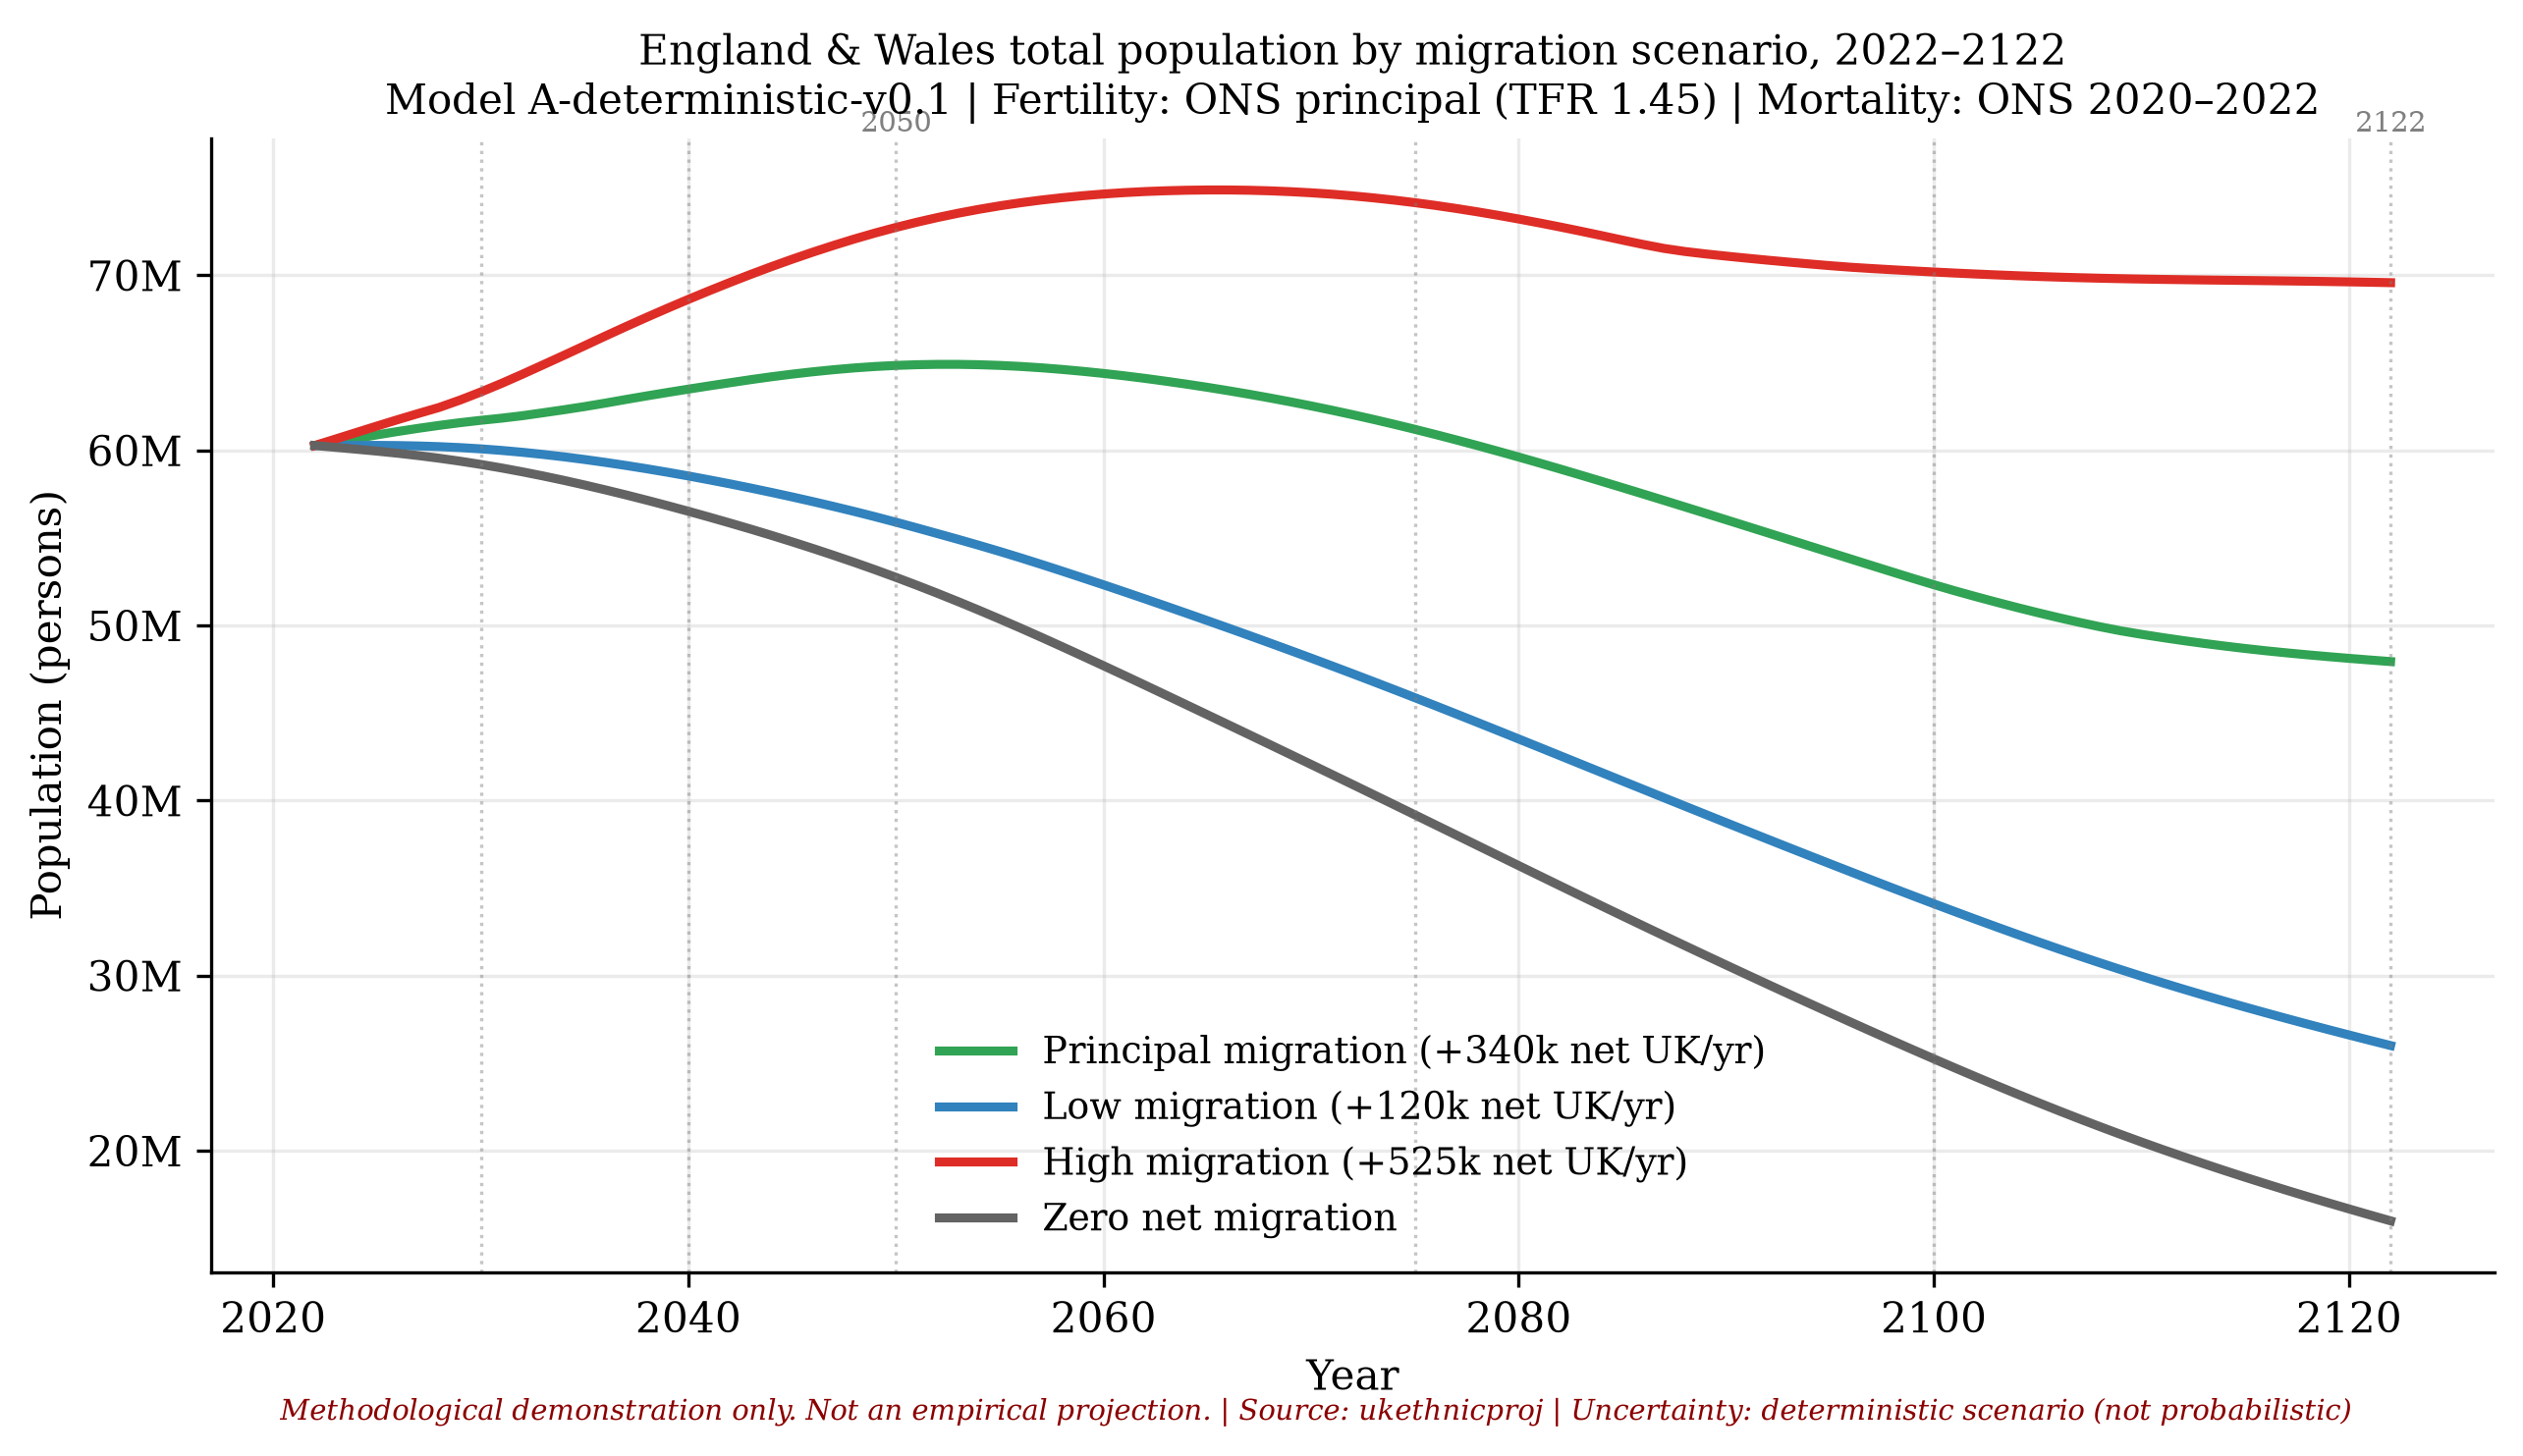
\includegraphics[width=0.95\textwidth]{../outputs/comparison/comparison_total_population.png}
\caption{Total England and Wales population under four ONS 2022-based migration scenarios,
2022--2122. Fertility and mortality held constant; migration is the only varying input.
\emph{Conditional projection only; not a forecast.}}
\label{fig:comparison_pop}
\end{figure}

\begin{figure}[H]
\centering
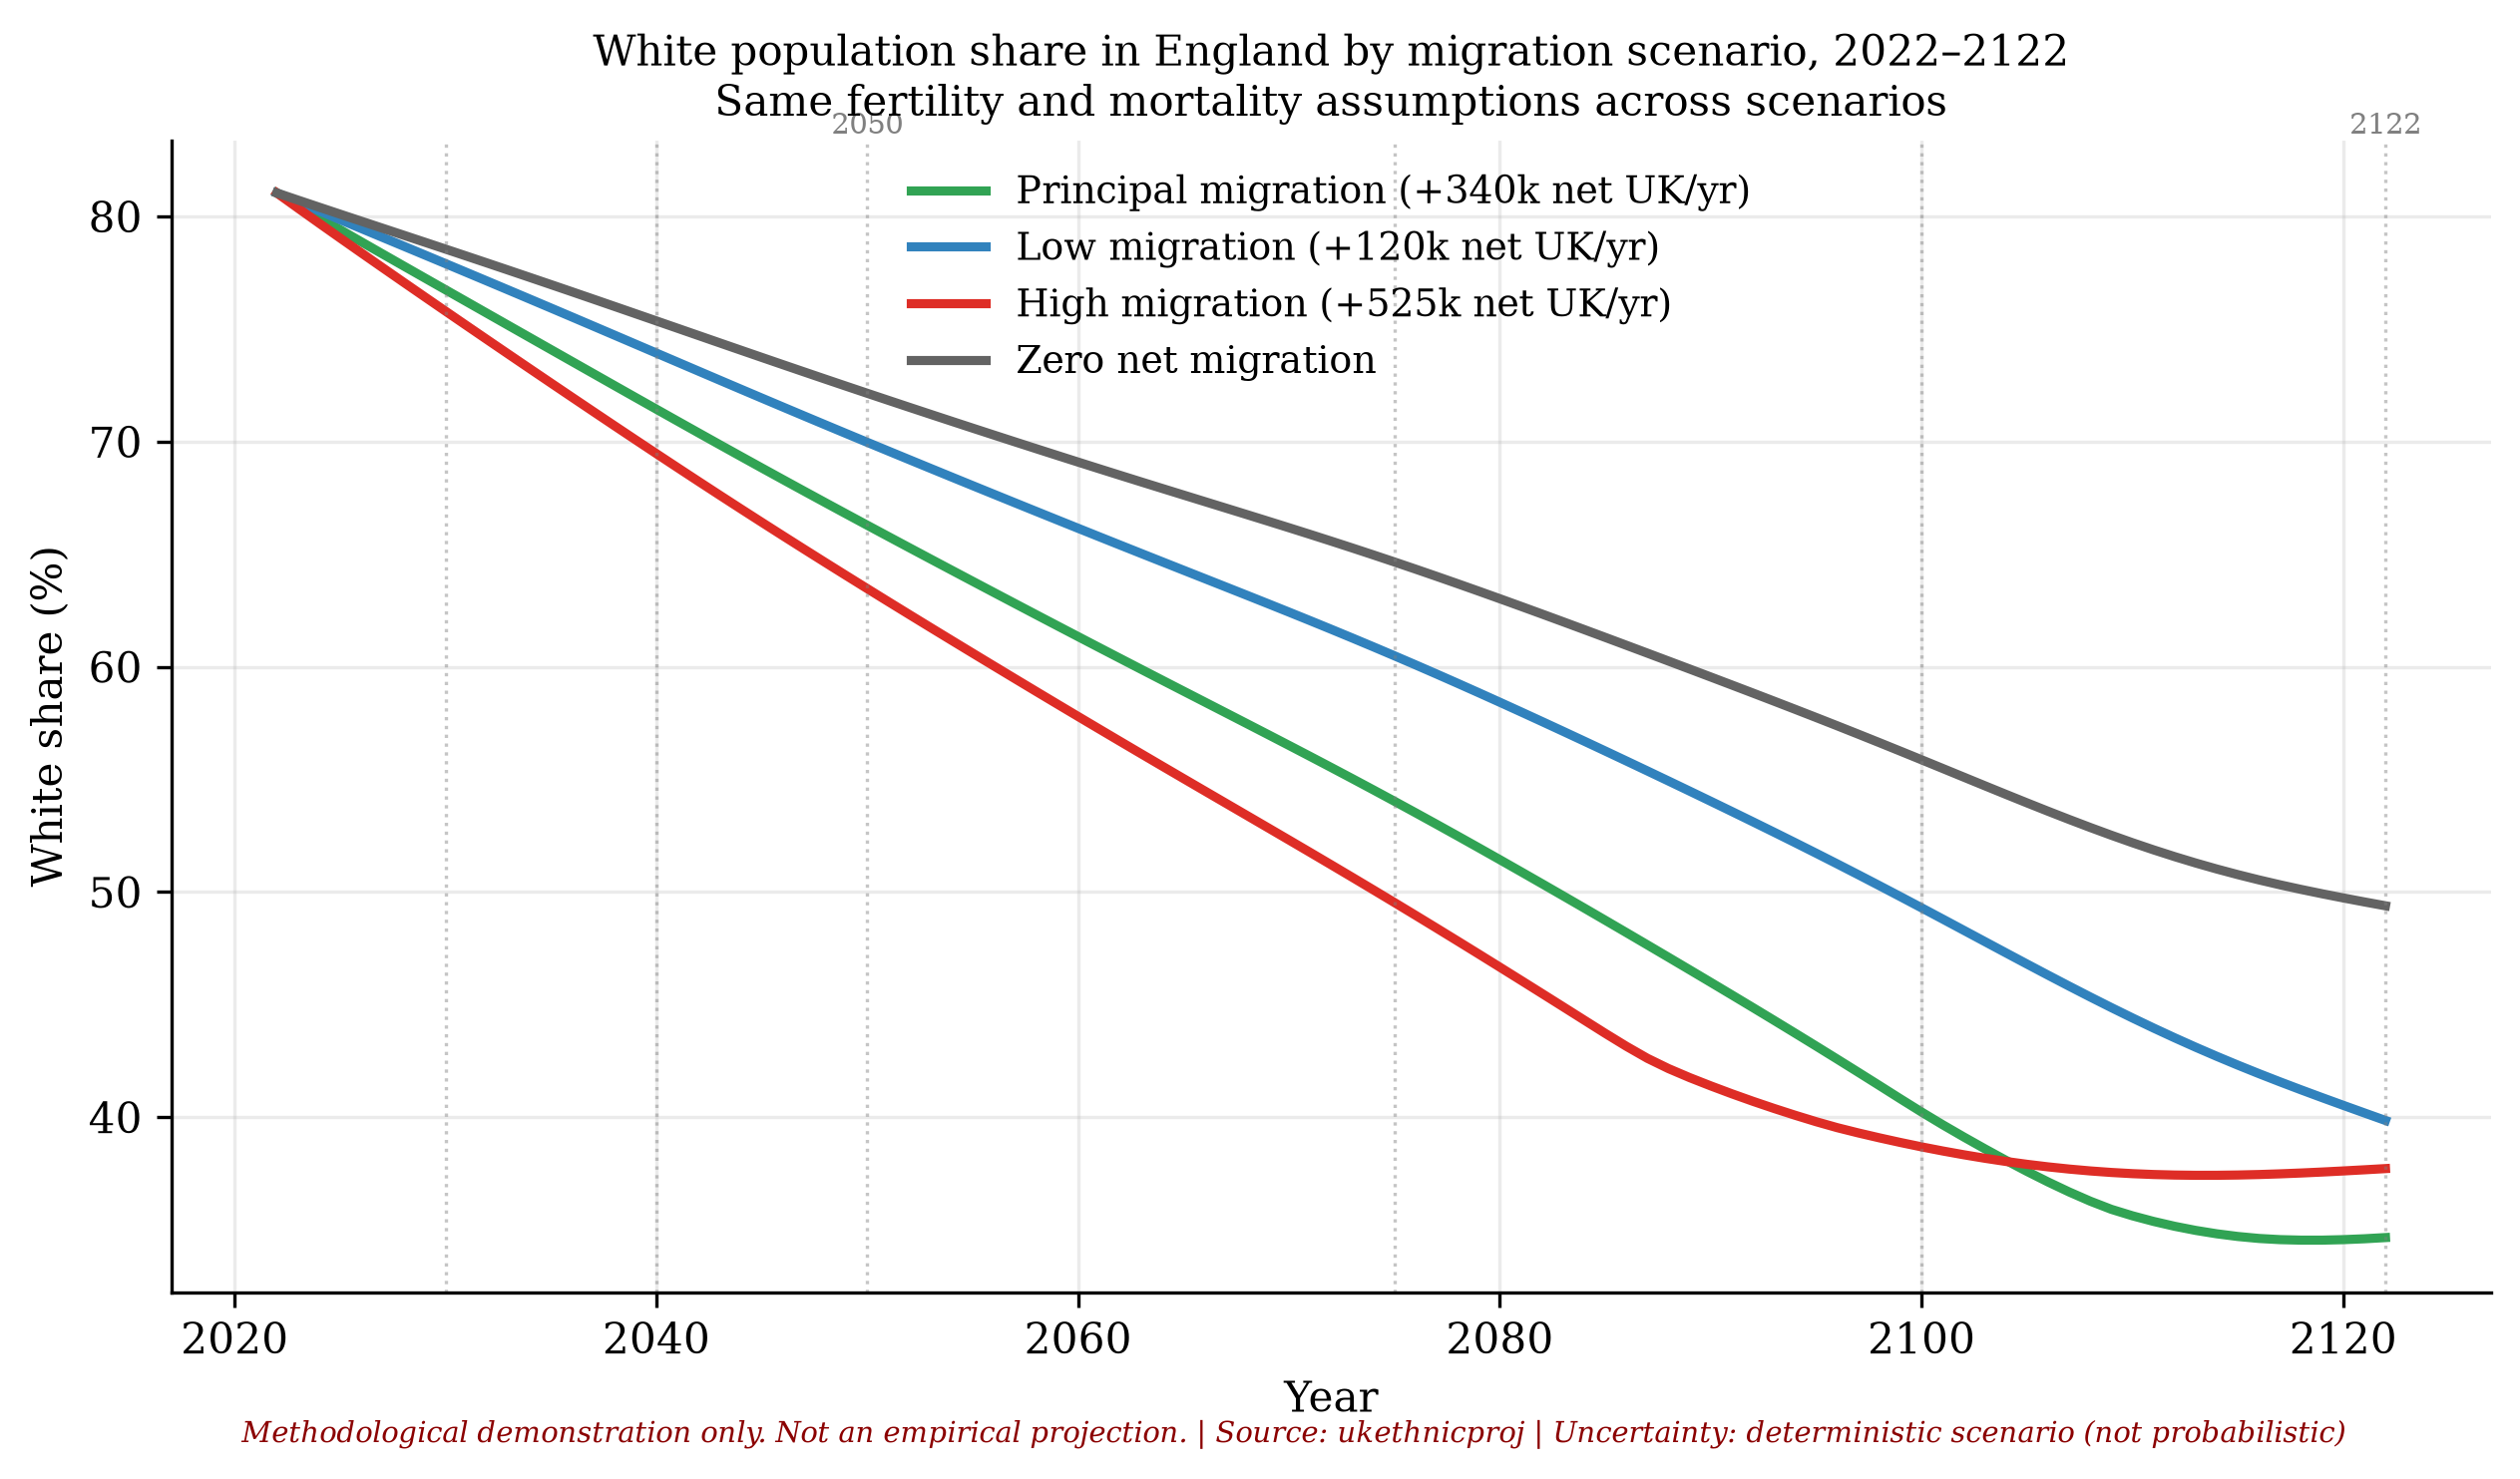
\includegraphics[width=0.95\textwidth]{../outputs/comparison/comparison_white_share_england.png}
\caption{White population share in England under four migration scenarios, 2022--2122.
Higher net migration produces faster diversification of ethnic composition under the
calibrated parameter set.}
\label{fig:comparison_white}
\end{figure}

\begin{figure}[H]
\centering
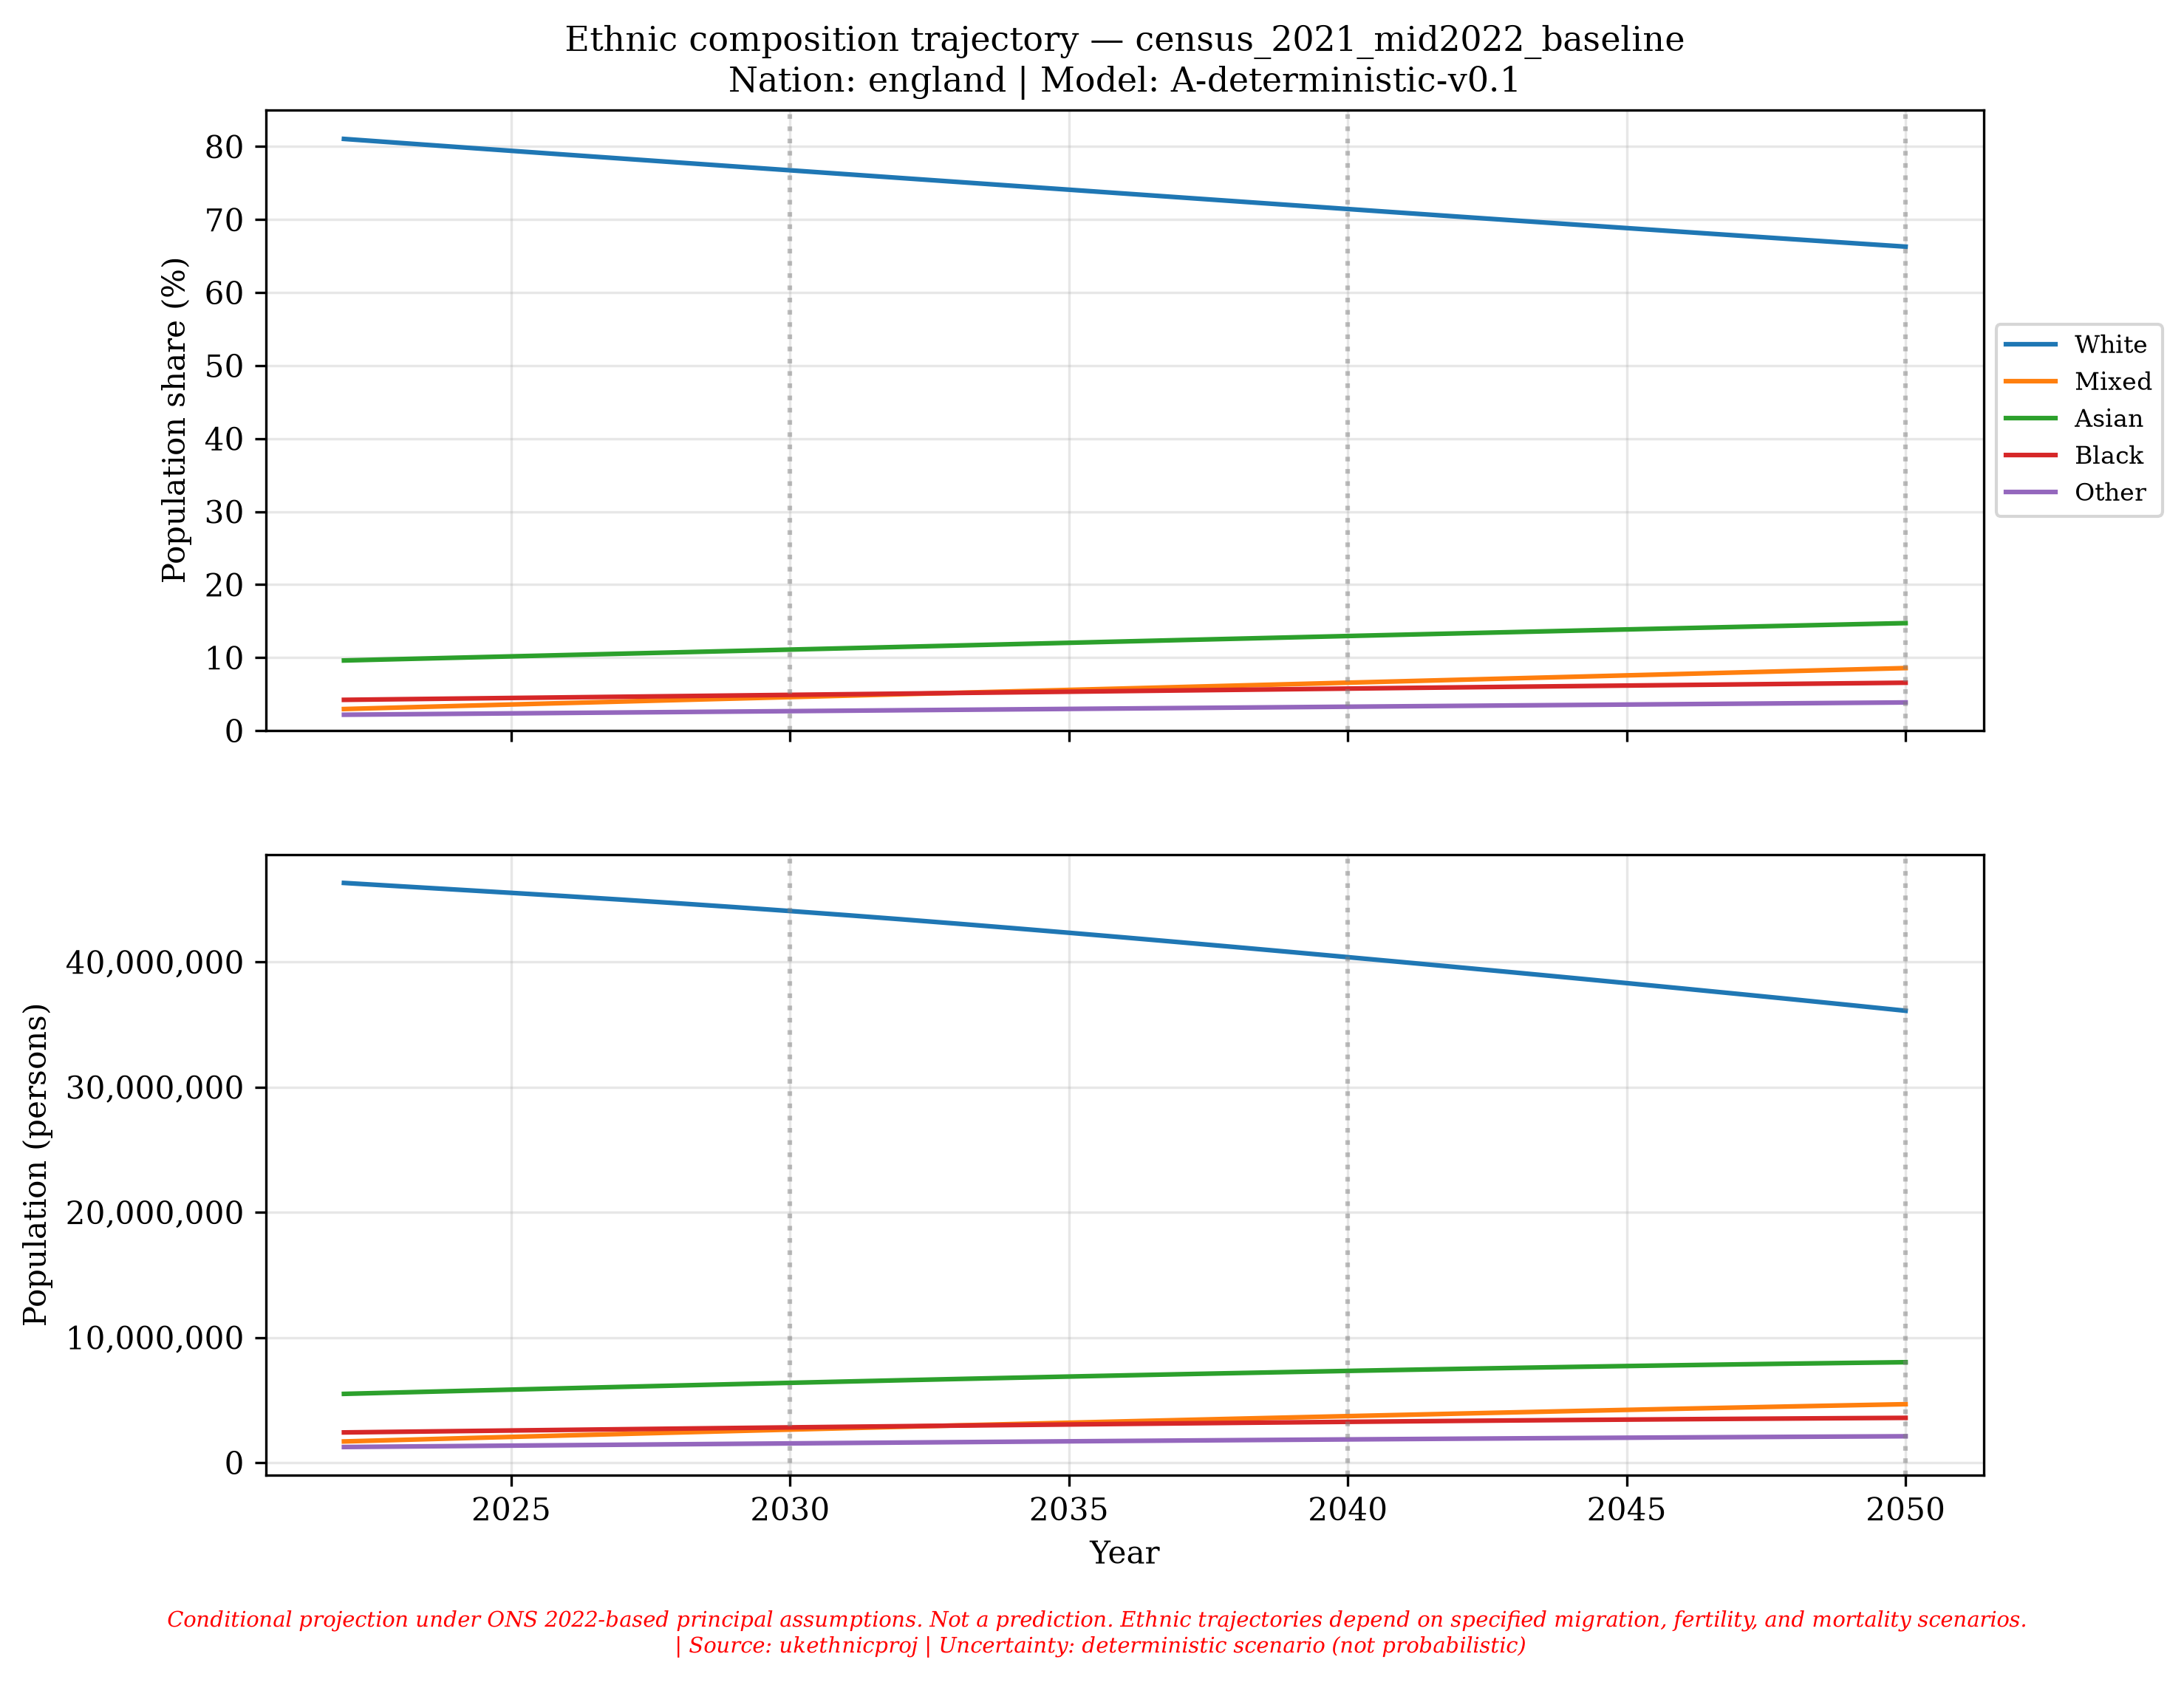
\includegraphics[width=0.98\textwidth]{../outputs/census_2021_mid2022_baseline/ethnic_shares_trajectory.png}
\caption{Ethnic population shares and counts in England under the principal ONS 2022-based
migration variant (Census 2021 base, mid-2022), 2022--2122. Wales is included in population
totals but excluded from share panels. \emph{Conditional projection only; not a forecast.}}
\label{fig:baseline}
\end{figure}

\begin{figure}[H]
\centering
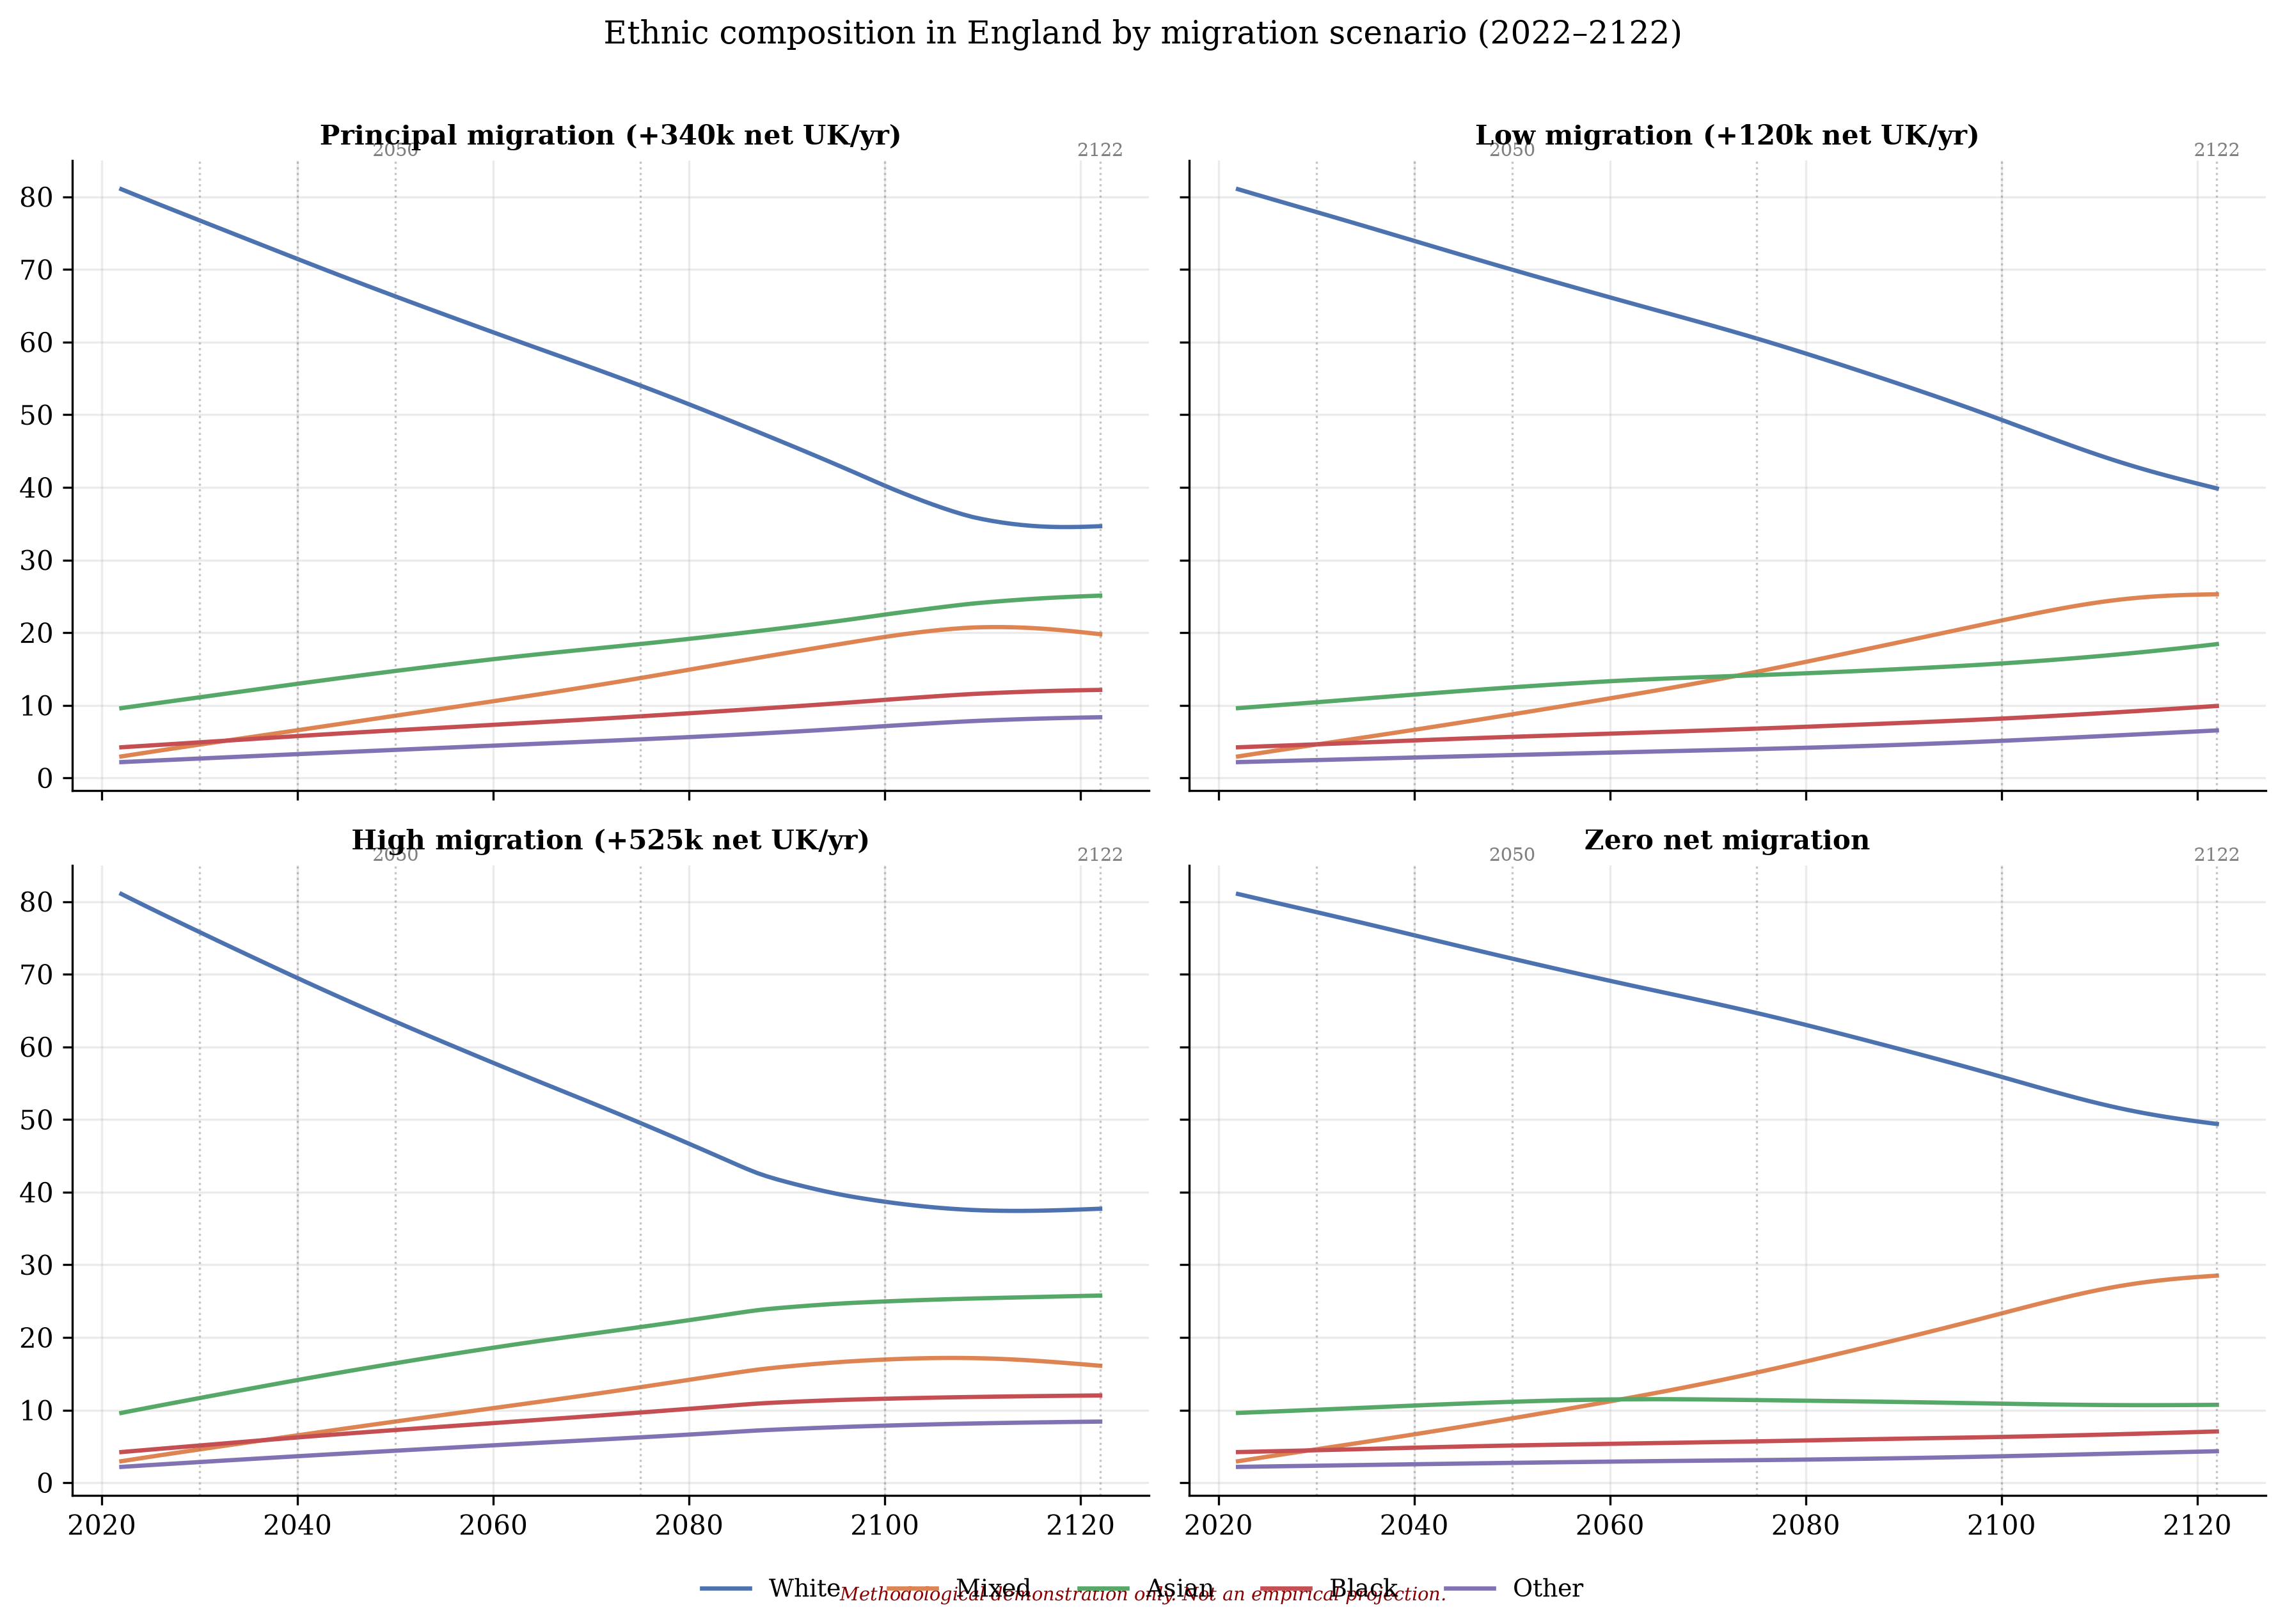
\includegraphics[width=0.98\textwidth]{../outputs/comparison/comparison_ethnic_shares_panel.png}
\caption{Ethnic composition in England by migration scenario (small multiples), 2022--2122.
Each panel shows the same five ethnic groups under a different ONS migration variant.}
\label{fig:comparison_panel}
\end{figure}

Figures~\ref{fig:comparison_pop}--\ref{fig:comparison_panel} show that migration assumptions
dominate both population scale and ethnic composition trajectories, consistent with prior UK
ethnic projection literature \citep{coleman2010, wohland2010}. The model does not attribute
causal policy effects; it reports arithmetic consequences of specified demographic inputs.
Long-horizon outputs to 2122 remain conditional and unvalidated---historical hindcasts are
required before treating century-scale trajectories as empirically credible forecasts.

\section{What this study can and cannot say}

\textbf{Can say:}
\begin{itemize}
    \item Under ONS 2022-based principal migration assumptions, a transparent cohort-component
    model starting from Census 2021 projects a mid-century peak of 64.9 million England and
    Wales residents (2050), with White share in England falling to 34.7\% by 2122 under the
    same assumptions.
    \item Migration scenario choice materially affects both population scale and ethnic
    composition; the 2122 population range spans 16.0--69.6 million across ONS variants.
    \item The pipeline is reproducible: all inputs are official aggregate tables with cached
    API responses and checksums.
\end{itemize}

\textbf{Cannot yet say:}
\begin{itemize}
    \item How ethnic composition will evolve to 2122 with \emph{validated} accuracy (hindcast
    not yet completed).
    \item Which assumptions contribute most to uncertainty (probabilistic mode not implemented).
    \item Whether the model would have projected Census 2011 or 2021 correctly (no hindcast).
    \item Results for Scotland, Northern Ireland, or the full UK total.
    \item That aggregate population totals match ONS principal NPP outputs (this model uses
    ONS migration volumes but not the full ONS projection system).
    \item Effects of specific immigration policy reforms (scenarios are demographic, not policy models).
\end{itemize}

\section{Conclusion}

This paper specifies and implements a reproducible ethnic population-projection system for
England and Wales, calibrated from Census 2021 and ONS/Nomis official statistics. Under
ONS 2022-based migration variants, conditional trajectories to 2122 show substantial
sensitivity of both population scale and ethnic composition to migration assumptions---a
finding consistent with prior UK ethnic projection research \citep{coleman2010, wohland2010}.
Mid-century results (e.g.\ 64.9 million under principal migration in 2050) are more informative
than century-scale totals until hindcast validation is complete.
The system treats ethnicity as self-identified and changeable, models immigration and
emigration separately, and enforces population accounting identities at each annual step.

Three principles govern interpretation. First, all results are \emph{conditional}: they
answer specified ``what if'' questions rather than predicting outcomes. Second, migration
assumption choice dominates long-run ethnic composition under the calibrated parameter set.
Third, credibility for longer horizons requires hindcast validation and fuller UK coverage
before substantive claims about 2122 are warranted.

Before such claims, historical hindcasts, Scotland and Northern Ireland integration,
partnership-based fertility, and probabilistic uncertainty quantification must be completed.
Until then, outputs should be read as formally specified demographic scenarios rather than
forecasts of the United Kingdom's future ethnic composition.

\section*{Data and code availability}

Source code, scenario configurations, harmonisation tables, and data manifests are available at\\
\url{https://github.com/sbf-developer/UK-Demographic-Change-Under-Alternative-Migration-and-Demographic-Scenarios-2022-2122}.
Raw API responses are cached with SHA-256 checksums under \texttt{data/raw/}. Census microdata
are not used; all inputs are aggregate official tables under the Open Government Licence v3.0.
Reproduction requires: \texttt{python -m ukethnicproj data fetch}, \texttt{calibrate},
\texttt{build-base-population}, and \texttt{simulate --scenario}.

\section*{Funding and conflicts of interest}

This is unfunded independent research. The author declares no conflicts of interest.

\section*{Acknowledgements}

Official data are provided by the Office for National Statistics, National Records of Scotland,
and the Northern Ireland Statistics and Research Agency under the Open Government Licence.

\bibliographystyle{apalike}
\begin{thebibliography}{99}

\bibitem[Coleman(2010)]{coleman2010}
Coleman, D. (2010).
Projections of the ethnic minority populations of the United Kingdom 2006--2056.
\emph{Population and Development Review}, 36(3), 441--486.
DOI: 10.1111/j.1728-4457.2010.00342.x

\bibitem[Haskey(2002)]{haskey2002}
Haskey, J. (2002).
Population projections for ethnic minority groups.
\emph{Population Trends}, 107, 24--32.

\bibitem[NEWETHPOP(2013)]{newethpop}
Rees, P., Wohland, P., \& Norman, P. (2013).
\textsc{NewEthPop}: Ethnic group population projections for UK local areas.
UK Data Archive SN 852508. \url{http://www.ehtnopop.org/}

\bibitem[ONS(2021)]{ons2021ethnicity}
Office for National Statistics. (2021).
\emph{Harmonised Concepts and Questions: Ethnic Group}.
GSS harmonisation guidance.

\bibitem[ONS(2023)]{ons2023rm032}
Office for National Statistics. (2023).
\emph{Census 2021: Ethnic group by sex by age (RM032)}.
Dataset RM032, Edition 2021, Version 1.

\bibitem[ONS(2024a)]{ons2024abme}
Office for National Statistics. (2024).
\emph{Long-term international migration, admin-based migration estimates}.

\bibitem[ONS(2024b)]{ons2024npp}
Office for National Statistics. (2024).
\emph{National population projections, 2022-based}.

\bibitem[ONS(2024c)]{ons2024nppmigration}
Office for National Statistics. (2024).
\emph{National population projections, migration assumptions: 2022-based}.

\bibitem[ONS(2024d)]{ons2024nppvariants}
Office for National Statistics. (2024).
\emph{National population projections, variant projections: 2022-based}.

\bibitem[ONS(2024e)]{ons2024lifetables}
Office for National Statistics. (2024).
\emph{National life tables, United Kingdom: 2020 to 2022}.

\bibitem[Rees et al.(2011)]{rees2011}
Rees, P., Wohland, P., Norman, P., \& Lomax, N. (2011).
The output population database: A method for flexible population forecasting.
\emph{Journal of Population Research}, 28(2--3), 167--184.

\bibitem[Rees et al.(2017)]{rees2017}
Rees, P., Wohland, P., Norman, P., \& Lomax, N. (2017).
Population projections by ethnicity: Challenges and a solution for the United Kingdom.
In D.~A. Swanson (Ed.), \emph{The Frontiers of Applied Demography} (pp.~383--408). Springer.

\bibitem[Wohland et al.(2010)]{wohland2010}
Wohland, P., Rees, P., Norman, P., Boden, P., \& Jasinska, K. (2010).
Ethnic population projections for the UK and local areas, 2001--2051.
University of Leeds School of Geography Working Paper 10/02.

\end{thebibliography}

\end{document}
